% Generated by manuscript/build_manuscript.py.
\section{Introduction}
\label{sec:introduction}


Multi-horizon forecasts support decisions over multiple planning ranges, from short-term control to long-term scheduling \citep{zeng2023dlinear}. Yet most long-term time-series forecasting models and benchmark protocols remain horizon-specific: a separate model is trained for each forecast horizon $H$, such as 96, 192, 336, and 720 steps \citep{nie2023patchtst,liu2024itransformer}. Recent work, including ElasTST\citep{zhang2024elastst} and time-series foundation models such as TimesFM\citep{das2024timesfm}, has begun to support varied or flexible forecasting horizons through autoregressive and universal-generation designs\citep{liu2024timer,ansari2024chronos,woo2024moirai}, with Time-MoE\citep{shi2025timemoe} providing a recent scalable example. Related work on coherent forecasting across temporal hierarchies likewise motivates coordinated decisions at short-, medium- and long-term planning levels \citep{rangapuram2023coherent}. However, these efforts remain sparse relative to the extensive horizon-specific literature and have not yet established varied-horizon forecasting as an explicit task with systematic problem analysis and targeted decoder design. In this work, we investigate how the decoder should organize output-side representations across different parts of the future domain.

The horizon-specific protocol fragments forecasting into independent predictors. As illustrated in Fig.~\ref{fig:conceptual-problems}a, models trained for different horizons can assign different values to the same future time step, despite identical history and forecast origin. Their outputs can therefore disagree on overlapping future targets rather than form nested views of a common trajectory. Supporting several horizons further entails separate training, checkpoint storage, deployment and maintenance.

We define \textbf{unified varied-horizon forecasting (UVHF)} as the setting in which one model serves different request endpoints through a shared prediction trajectory. Formally, UVHF learns a single horizon-agnostic mapping from observed history and future-step index to prediction. Under this mapping, a future-step prediction depends on the history and its step index, but not on the requested horizon. For any $H_1<H_2$, predictions over steps $1{:}H_1$ therefore remain identical under both requests. We call this requirement \textbf{cross-horizon prefix consistency (CHPC)}.

CHPC specifies how forecasts at different horizons should relate, but not how a decoder should generate different future regions. Most architectural advances focus on history encoding, while the output stage often uses a uniform mechanism for all future steps \citep{zhou2021informer,wu2021autoformer,zhou2022fedformer,liu2022nonstationary}. Such a decoder fixes the sharing extent, that is, how broadly a history-conditioned latent state is reused before step-specific generation. Broad sharing can capture persistent trajectory structure but may smooth local variations. Finer sharing offers greater step-specific flexibility but weaker structural regularization. The preferred balance can vary across samples, variables and future regions, making a fixed extent inadequate for the full forecast domain. Fig.~\ref{fig:conceptual-problems}b summarizes this output-side heterogeneity, which we term \textbf{future-region sharing-demand heterogeneity}. We examine this problem in greater detail in Section~\ref{sec:problem-formulation}.



\begin{figure*}[t]
\centering
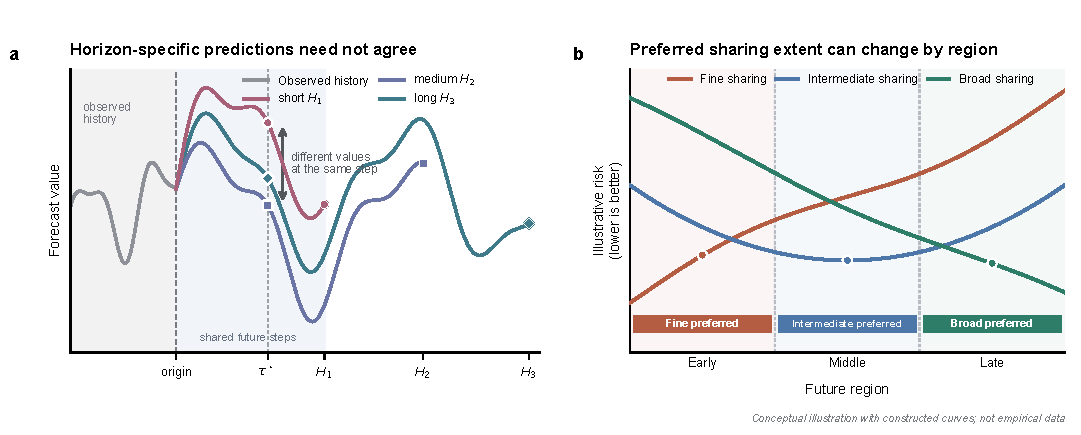
\includegraphics[width=1.00\textwidth]{figures/figure_01_conceptual_problem.pdf}
\caption{Two challenges in unified varied-horizon forecasting. \textbf{a}, Horizon-specific predictors may disagree at the same future time step $\tau^\star$ despite identical observed history. \textbf{b}, The sharing extent associated with the lowest risk can vary across future regions.}
\label{fig:conceptual-problems}
\end{figure*}


Motivated by this heterogeneity, we propose HoriScope, an adaptive multi-scope decoder that integrates forecasts generated under different sharing extents. HoriScope assigns each scope a dedicated history projection within one scope-indexed forecast field. Each scope specifies how broadly a history-conditioned latent state is reused before step-specific generation. A single-scope decoder fixes this extent throughout the forecast domain. HoriScope instead allocates scope-conditioned forecasts for each sample, variable and future step. The resulting trajectory can adapt its sharing composition across future regions while retaining a single horizon-agnostic prediction function. To support joint learning, Balanced Scope Co-Adaptation (BSCA) supplies direct prediction signals to all scopes and discourages premature allocation concentration. BSCA operates only during training, adds no inference parameters or paths, and preserves CHPC across supported horizons.

The contributions of our work are summarized as follows:

\begin{enumerate}
\item We formulate UVHF as a forecasting system in which CHPC is a basic requirement, and identify future-region sharing-demand heterogeneity as an output-side challenge.
\item We introduce HoriScope, which integrates forecasts generated under multiple sharing scopes through target-adaptive allocation.
\item We develop BSCA to support balanced scope learning without increasing inference-time complexity.
\end{enumerate}

Experiments across datasets from multiple application domains show that a single unified model outperforms separately trained horizon-specific forecasters. Component-wise ablations support the utility of the proposed components, and generalization studies demonstrate decoder portability across the evaluated backbone families.
